\section{Scelta della camera}
Inizialmente si è scelta come camera \textit{SpotLight Pro Webcam}, una webcam già utilizzata in un progetto precedente \textit{Trust} (fig. ~\ref{fig:TrustCam}).
\begin{figure}[H]
	\centering
	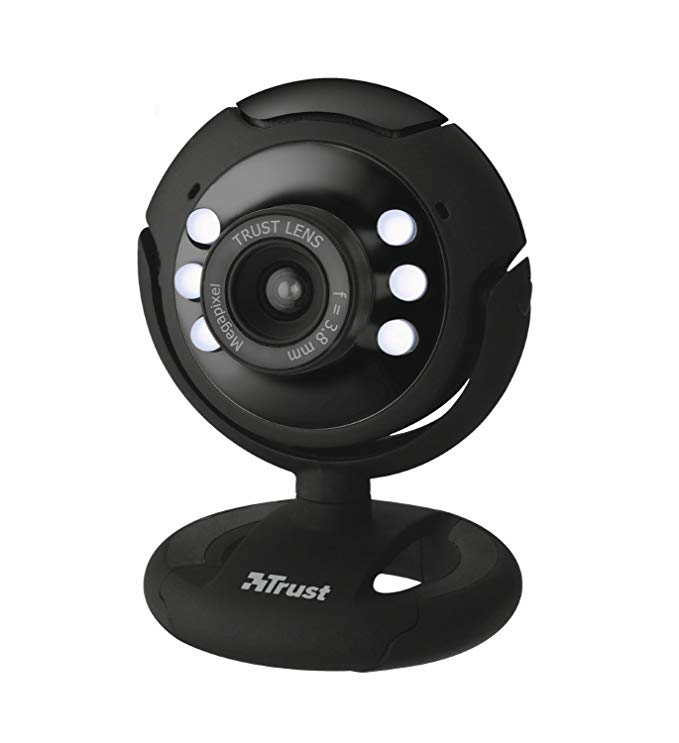
\includegraphics[width=0.3\textwidth]{Immagini/TrustCam.jpg}
	\caption{Camera utilizzata inizialmente}
	\label{fig:TrustCam}
\end{figure}
È stato però notato che, questa camera, non era in grado di dare sufficienti garanzie di funzionamento stabile in alcune delle più comuni condizioni luminose.

Si è deciso quindi di passare ad una camera di tipo industriale, in grado di fornire delle prestazioni più stabili e affidabili. 
La scelta è ricaduta sulla camera della casa produttrice \textit{IDS (Imaging Development System)}: si tratta del modello \textit{UI-1221LE-C-HQ} equipaggiata con la lente \textit{BM2420} della casa \textit{Lensagon}.
\begin{figure}[H]
	\centering
	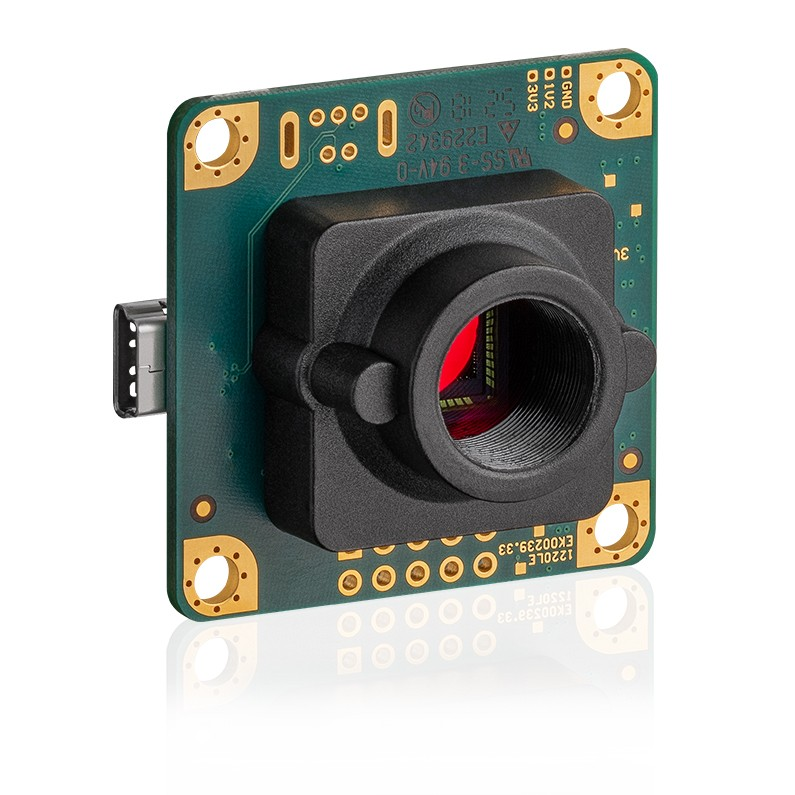
\includegraphics[width=0.3\textwidth]{Immagini/camera-usb2-ueye-le-rev2-boardlevel-m12-1.jpg}
	\caption{Camera utilizzata successivamente}
	\label{fig:Cam}
\end{figure}

La camera in Fig.\ref{fig:Cam} ha un'otturatore globale che permette di acquisire tutta l'immagine istantaneamente e non in modo progressivo come la camera  \textit{SpotLight Pro Webcam}



\section{Vericale o orizzontale?}
TODO che vuol dire?
\section{Come ottenere le immagini dalla camera?}
Per ottenere le immagini dalla camera è stato necessario iscriversi presso il sito web della casa produttrice e scaricare i driver necessari all'installazione.
La videocamera ha diverse opzioni di acquisizione tra cui anche una grandezza dell'immagine diversa dal classico 480x640 ma per ragioni di semplicità si è scelto di lasciare invariate le impostazioni di default.

\section{CPU consumption}
Un fattore importante nella scelta della camera è l'elevato tempo di utilizzo della CPU da parte della camera \textit{UI-1221LE-C-HQ}. In contrasto, la camera inizialmente scelta vantava un consumo di CPU nettamente inferiore e quindi che più si potrebbe adattare all'installazione su dispositivi mobili e con bassa potenza di calcolo.

\section{Installazione}

Durante i test e gli esperimenti svolti in laboratorio la videocamera è stata legata ad un palo metallico e fissata con un angolo di inclinazione rispetto ad esso di circa 35 gradi; l'altezza dal pavimento era, inoltre, di 83.5 cm

